\documentclass[border=0mm]{standalone}
\usepackage{tikz}
\usepackage{amsmath}
\usepackage{amsmath}
\usetikzlibrary{calc, angles, quotes}
\begin{document}
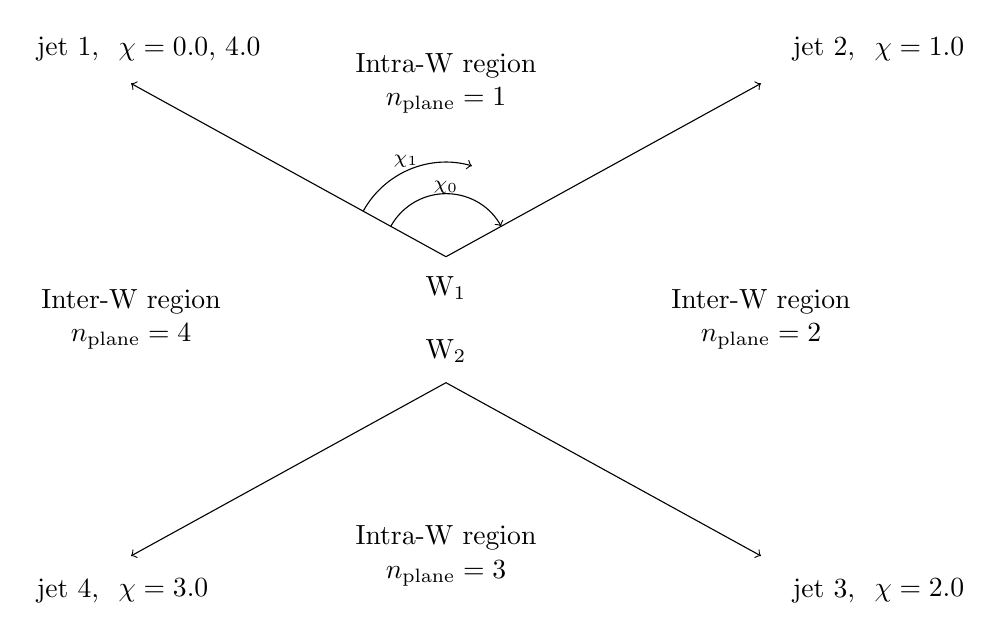
\begin{tikzpicture}
  \coordinate(W1) at (0, 0.8);
  \coordinate(W2) at (0, -0.8);
  \coordinate(c1) at (-4, 3);
  \coordinate(c1a) at (0.2, 1.5);
  \coordinate(c2) at (4, 3);
  \coordinate(c3) at (4, -3);
  \coordinate(c4) at (-4, -3);
  \begin{scope}[local bounding box = inset]

    \draw[->] (W1) -- (c1);
    \draw[->] (W1) -- (c2);
    \draw[->] (W2) -- (c3);
    \draw[->] (W2) -- (c4);
    \draw[<-] pic [draw, angle radius=1.2cm, angle eccentricity=1.1,"$\chi_{1}$" font=\scriptsize] {angle=c1a--W1--c1};
    \draw[<-] pic [draw, angle radius=0.8cm, angle eccentricity=1.1,"$\chi_{0}$" font=\scriptsize] {angle=c2--W1--c1};

  \end{scope}
  \node(b1)[align = center] at (inset.north)[anchor=center]{
    Intra-W region\\
    $n_\text{plane}=1$
  };

  \node(b2)[align = center] at (inset.east)[anchor=center]{
    Inter-W region\\
    $n_\text{plane}=2$
  };

  \node(b3)[align = center] at (inset.south)[anchor=center]{
    
    Intra-W region\\
    $n_\text{plane}=3$
  };

  \node(b4)[align = center] at (inset.west)[anchor=center]{
    Inter-W region\\
    $n_\text{plane}=4$
  };

  \node(t1) at ($(W1)!1.2!(c1)$) {jet 1,}; \node(t1chi) at (t1.east)[anchor=west]{$\chi=0.0$, $4.0$}; 
  \node(t2) at ($(W1)!1.2!(c2)$) {jet 2,}; \node(t2chi) at (t2.east)[anchor=west]{$\chi=1.0$};
  \node(t3) at ($(W2)!1.2!(c3)$) {jet 3,}; \node(t3chi) at (t3.east)[anchor=west]{$\chi=2.0$};
  \node(t4) at ($(W2)!1.2!(c4)$) {jet 4,}; \node(t4chi) at (t4.east)[anchor=west]{$\chi=3.0$};

  \node(l1) at ($(W1) - (0, 0.4)$) {$\text{W}_{1}$};
  \node(l2) at ($(W2) + (0, 0.4)$) {$\text{W}_{2}$};  
\end{tikzpicture}
\end{document}
